\section{Solution}

In this section, we present the identified research gaps, an overview of the proposed solution, and the innovative aspects of this solution. The proposed solution aims to contribute to the application of Deep Reinforcement Learning (DRL) in Forex trading by addressing specific research gaps and introducing novel approaches to model architecture, training, and optimisation techniques.

\subsection{Research Gaps}

Several research gaps have been identified. Firstly, the application of the Deep Deterministic Policy Gradient (DDPG) in Forex markets is underexplored, despite its advantages in handling continuous action spaces. Secondly, while Recurrent Neural Networks (RNN), especially Long-Short Term Memory (LSTM) networks, are effective for time-dependent data, their integration with DDPG in Forex trading remains limited. Thirdly, enhancing the reward function from total return to the Sharpe ratio for better risk-adjusted returns is needed. Furthermore, online learning for real-time market adaptation is relatively unexplored, and advanced risk and portfolio management techniques, such as variable position sizing within the DDPG framework, require further research.

\subsection{Proposed Solution}

The proposed solution addresses these gaps by developing a Forex trading system that integrates DDPG with an LSTM architecture, incorporates the Sharpe ratio as the reward function, and supports online learning for continuous market adaptation. This approach aims to leverage the strengths of advanced DRL techniques to enhance trading performance and robustness.

\subsubsection{Model Innovation}

The application of DDPG to the Forex market represents a significant innovation in this field. DDPG is at the forefront of advancements in DRL algorithms, known for its ability to handle high-dimensional continuous action spaces effectively, making it particularly suitable for complex trading environments. Initially, the model will be tested with fixed position sizing. However, given DDPG's capability to support continuous action spaces, we will explore the potential of variable position sizing to enhance trading strategies. The initial implementation will utilize a vanilla FNN underneath the DDPG model. If time permits, we plan to integrate an RNN (LSTM) architecture due to its superiority in capturing sequential dependencies and temporal patterns, which are critical in financial time series analysis. Moreover, we will begin with the total return as the reward function but aim to test the Sharpe ratio if feasible, due to its focus on risk-adjusted performance, offering a more comprehensive evaluation of trading strategies. This plan includes testing eight different models: DDPG with FNN and RNN (LSTM), each with fixed and variable position sizing, using both total return and Sharpe ratio as reward functions.

\subsubsection{Training Innovation}

A key innovative aspect of the proposed solution is the direct integration with the cTrader platform \cite{noauthor_forex_nodate}, a prominent trading platform supported by many well-known brokers and a major competitor to MetaTrader4/5 \cite{noauthor_metatrader_nodate}. cTrader’s cross-broker compatibility allows researchers to select brokers that best align with their requirements, such as commission rates, swaps, and spreads. This project proposes building a server in .NET and a client in Python, where the server handles data feeds and trading operations (e.g., opening, modifying, and closing positions), and the client processes these feeds and sends back trading decisions. This setup enables online training, a superior technique that closely simulates live trading conditions, allowing the model to adapt to real-time market changes. In addition, it facilitates visual backtesting of strategies and seamless deployment in live trading contexts. This approach aims to combine the robustness of cTrader’s infrastructure with the flexibility and analytical capabilities of Python, allowing accurate performance results that account for real explicit and implicit costs.

\subsubsection{Optimization Innovation}

The proposed solution introduces several innovative optimisation techniques to improve the convergence and generalisation power of the model. We will start by testing the model on an hourly timeframe for the 7 major Forex pairs, an underexplored area, and, if feasible, extend the testing to a daily timeframe. The state space will be enriched with technical analysis components in addition to OHLCV data to provide a comprehensive view of market conditions and achieve the Markov property, which is essential for effective reinforcement learning. All features will undergo rigorous engineering; we plan to apply normalisation techniques to standardise the data, making it easier for the neural networks to process and learn effectively. Regularisation techniques and adaptive learning rates will be used in neural network models to mitigate bias-variance issues, enhancing the generalisation capabilities of the model. In the reinforcement learning models, we will utilise \(\varepsilon\)-greedy policies and Gaussian noise to balance exploration and exploitation, encouraging the discovery of optimal trading strategies while leveraging known profitable actions. These optimisation strategies are designed to enhance the model's performance, stability, and adaptability, ensuring it can effectively navigate the complexities of the Forex market.

\subsubsection{System Architecture}

The system architecture diagram for the proposed solution is shown in Figure \ref{Figure:SystemArchitecture}. This architecture consists of three major components: the Market, the Server Manager and the Client Manager. In this framework, we are implementing a one-to-one Client-Server architecture, meaning that for each asset there is one Client that generates signals and one Server that handles the data feeds and positioning operations. Therefore, this is a one-to-one communication and there exist as many Servers as Clients. Then, each set of Servers and Clients is managed by a Server Manager and a Client Manager, respectively, capable of starting, monitoring and shutting all of them. Going in more depth on the details, firstly, the Market component represents a broker with access to the cTrader platform. There are currently several prestigious and regulated alternatives, but for this research we will use IC Markets EU as our broker \cite{noauthor_cfd_nodate}. Secondly, the Server Manager component represents a cTrader platform running on the local machine. Within cTrader platform there are several Servers running, where each one of them basically consists on a cBot implementation, a .NET program that allows algorithmic trading within cTrader. Each Server includes several submodules, namely: the Call module, which sends requests to the Client; the Live Position module, responsible for opening, modifying, and closing positions; and the Live Feeds module, which receives Tick and Bar data and checks how new data affected currently opened positions; and the Callback Handler module, which handles requests from the Client. Thirdly, the Client Manager component, implemented in Python, consists of a program that manages individual Clients, each one connected to a single server and with similar submodules to it, namely: the Callback module that receives data from the Server including Tick/Bar data and position information; the Feature Engineering module that cleans, normalises, standardises and adds technical analysis to the data; the DRL Model module, including a Neural Network submodule (either FNN or LSTM), a RL submodule (actor-critic), and a Reward Function submodule (Total Return or Sharpe Ratio), which receives the processed data and generates actions (long, short, neutral); and the Call module that sends these actions to the Server. Upon successful execution of actions by the Server, the Client waits for the reward, which is generated when positions are closed. This architecture ensures robust, real-time adaptation and performance evaluation of the DRL-based trading system in an online training paradigm.

\begin{figure}[htb!]
    \centering
    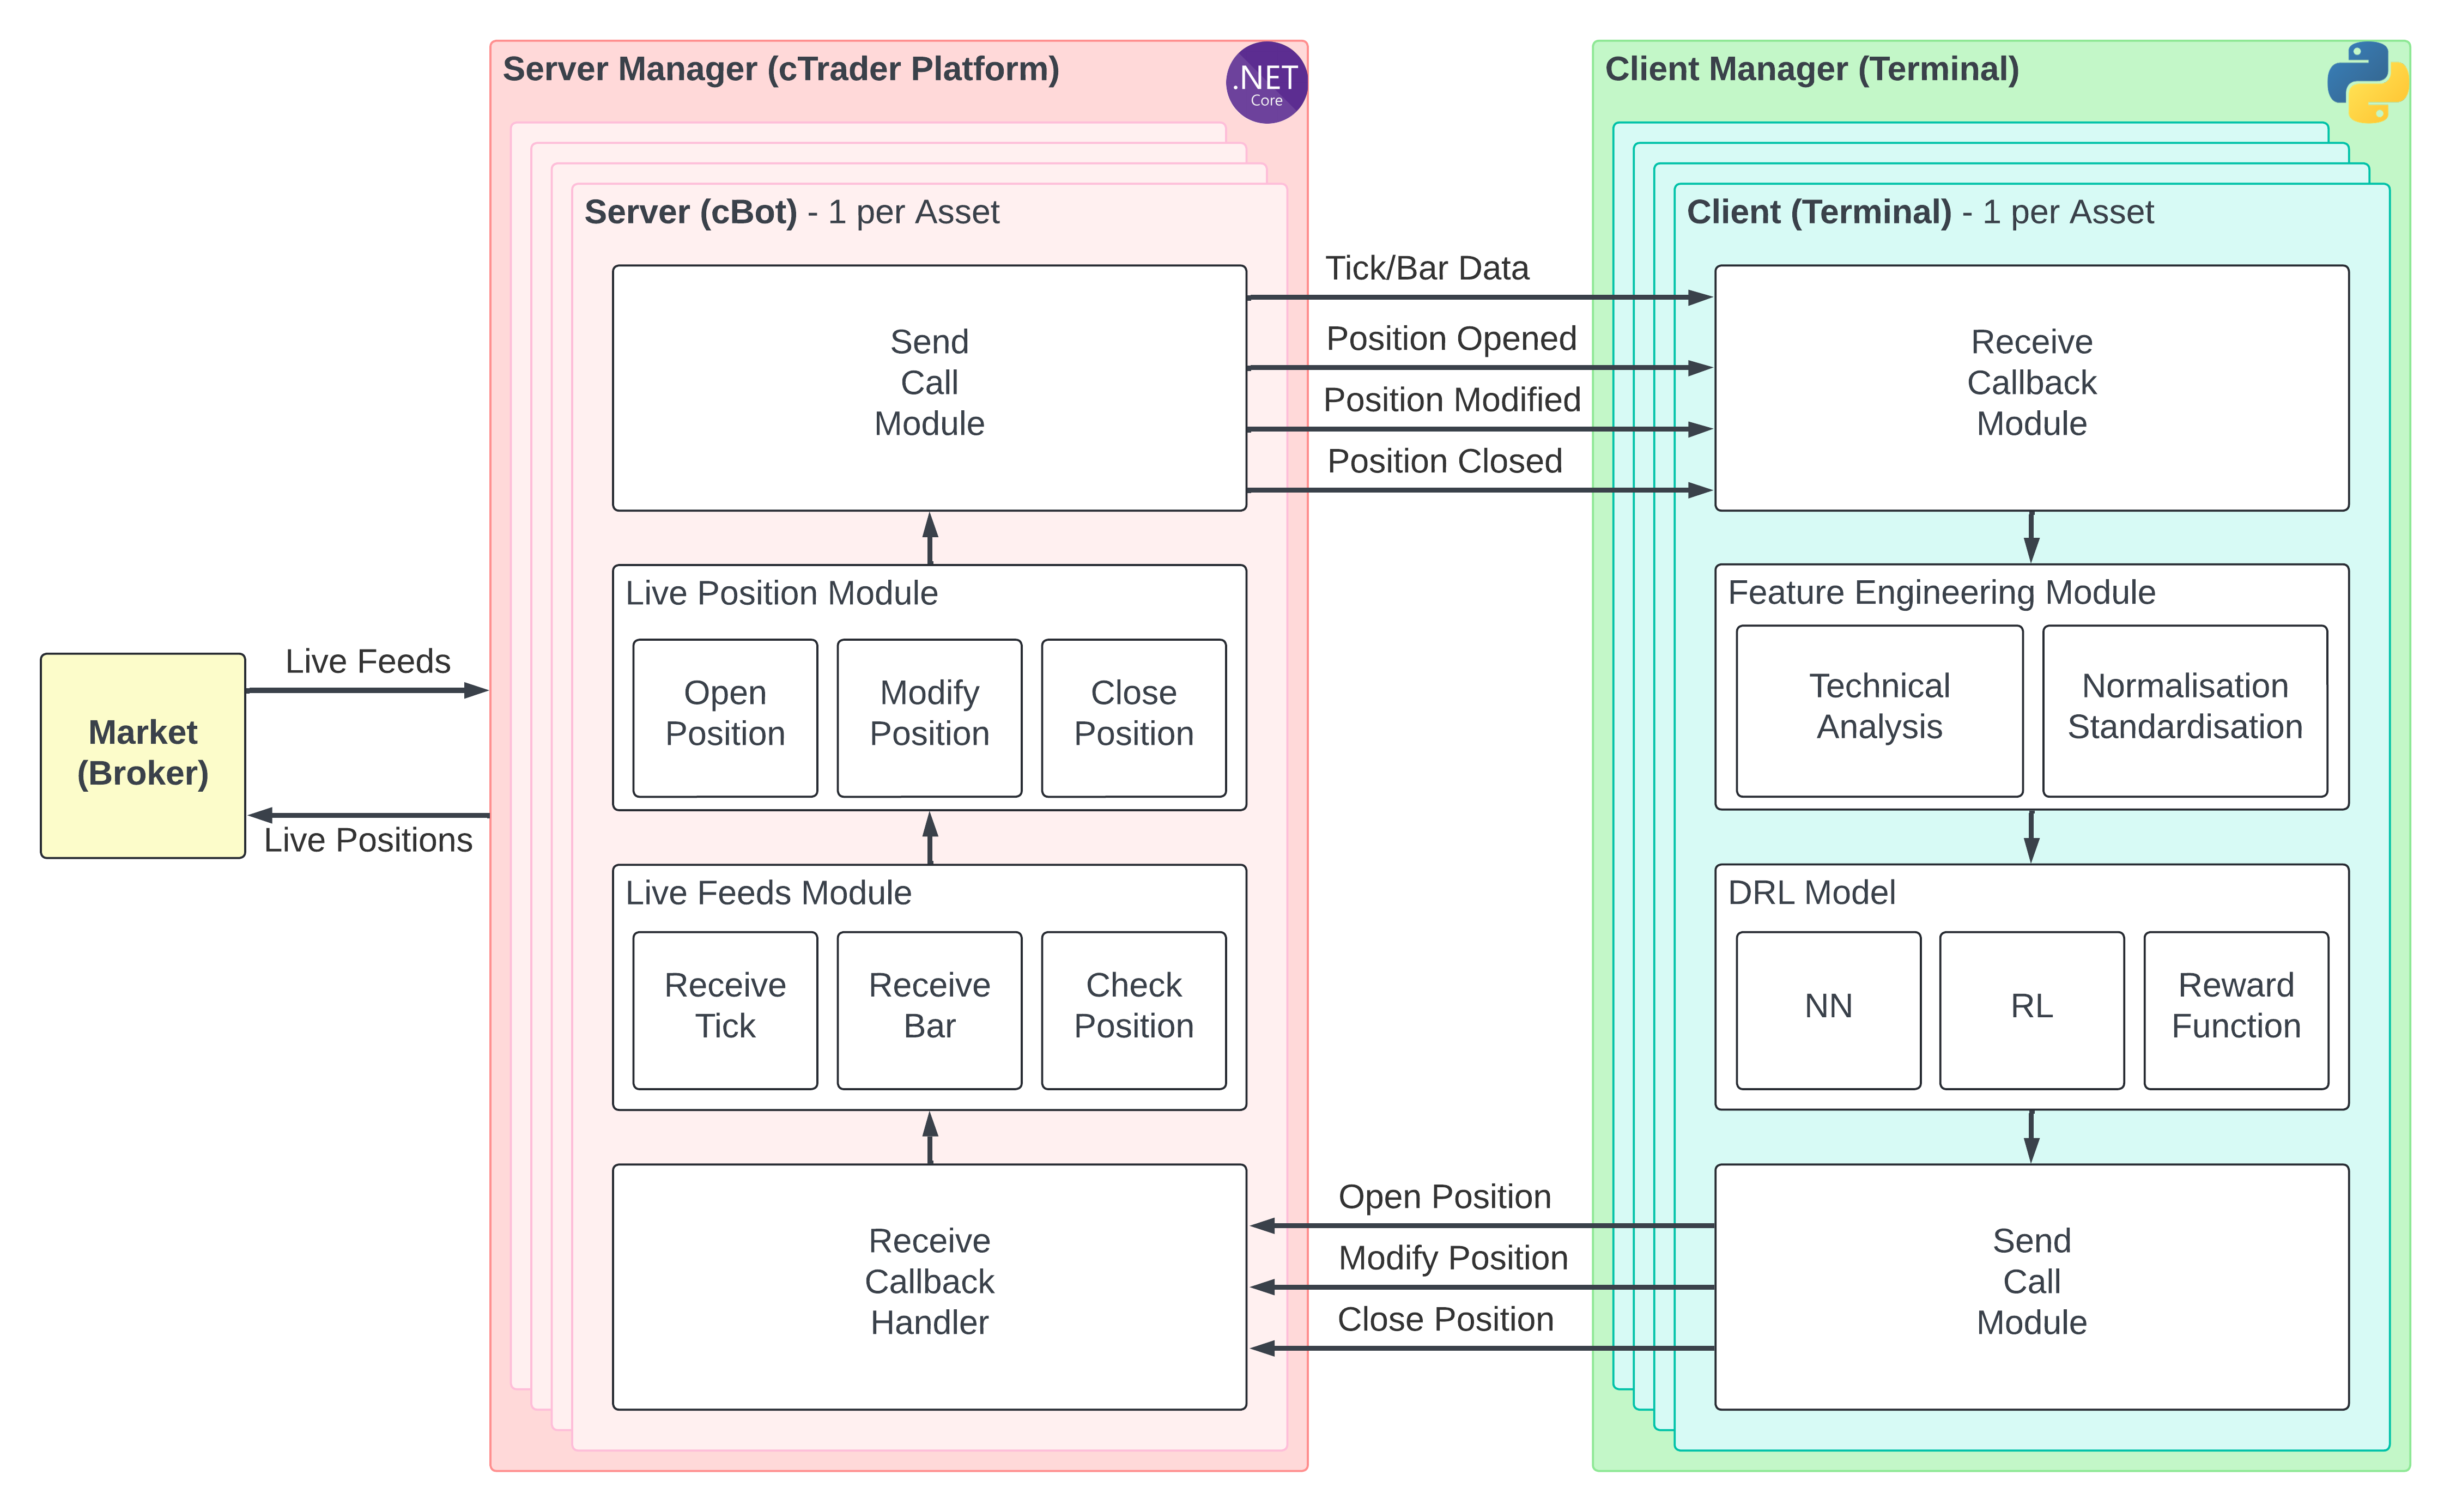
\includegraphics[width=\textwidth]{Images/SystemArchitecture.png}
    \caption{Proposed DRL-based Forex Trading System Architecture}
    \label{Figure:SystemArchitecture}
\end{figure}
